\section{From single-core CPUs over multi-core CPUs to GPUs}

\begin{figure} \label{fig_tree_reduction}
    \centering
    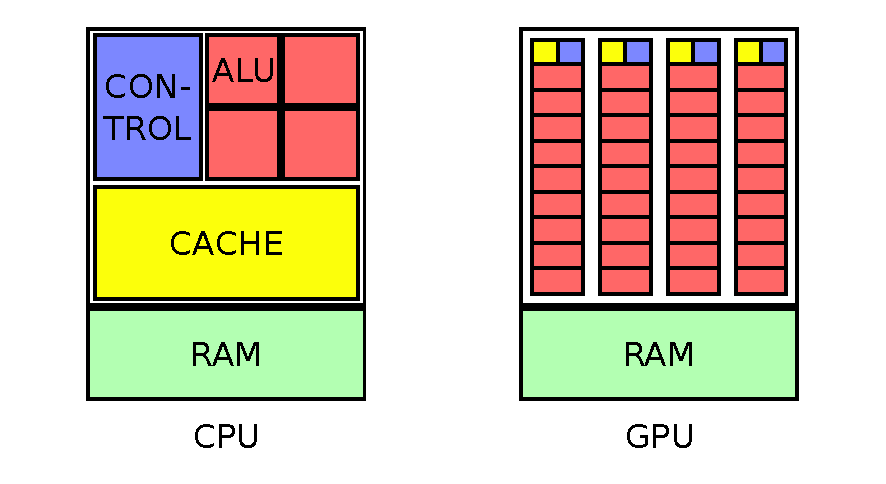
\includegraphics[]{cpu_vs_gpu.pdf}
    \caption{
        Comparison of the basic architectural differences of a GPU and a CPU.
        In green the random access memory (RAM), in yellow the cache, in blue the flow control unit and in red the arithmetic-logic unit (ALU).
        Both designs feature a RAM that all threads have access to.
        The GPU is split into many small "CPUs" (vertical groups) with their own flow control and cache.
        These are called streaming multiprocessors (SMPs or SMs).
        Generally the cache hierachry is more complicated as depicted in the figure.
        However, the defining property here is that there exists a non-global cache level that is assigned to a group of ALUs, namely the SMs. 
        Note that the notion of an ALU has slightly different meaning for a CPU and a GPU.
        For a CPU one ALU usually corresponds to one thread.
        For a GPU one ALU usually corresponds to a group of threads (for modern GPUs: 32), called a warp.
    }
\end{figure}

With the invention of the MOS transistor in 1959 and more specifically the silicon-gate MOS transistor in 1968 the development of single-chip microprocessors started.
The first processors were single-threaded and their bottleneck was (besides other things) their clock rate.
However, clock rates increased exponentially over time and subsequentially did the computing power.
In the 2000s this development was eventually brought to a halt at around 3.4 GHz due to thermodynamical limits of silicon. 
While pushing past that limit is possible, the extra costs for cooling usually outweight the increase in computing power.
This is the beginning of the multiprocessing era. 
The idea is simple: When one thread cannot run faster, just increase the number of threads.
In 2006 the first desktop PCs with two cores were sold and ever since the number of threads is steadily increasing.
There was one problem in particular, however, that CPUs (Central Processing Unit) were not efficient in solving, namely, rendering graphics.
This task required a lot of independent and small calculations that needed to be done in real time - a prime example for a massively parallelisable computation.
Since rendering graphics required such a different type of computing, the first GPUs (Graphics Processing Unit) were developed.
These GPUs featured less single thread computation power but have a higher number of threads.
State of the art GPUs have thousands of threads.
This being said, the number of threads cannot be easily compared between a CPU and a GPU or even between different GPUs as they follow different design paradigms.
How the GPU threads work exactly will be explored in this work.
Generally, one can say that GPUs perform well in massively parallelisable computations where the single computations are not complex while CPUs excel at complicated single threaded problems (for example running the event loop of a desktop application).
This shift to a higher number of threads rather than thread quality has been greatly motivated by scientific calculations, machine learning and graphics.

In this work, the basics of GPU programming in CUDA will be introduced and a very important algorithm presented, namely the tree reduction.
Using this algorithm as an example, a deeper look into the architecture of GPUs and the CUDA programming language will bring forth various optimisations.
Finally, the highly optimized implementation of the tree reduction will be tested on a consumer grade setup and a high-performance computer and the results will be discussed.

\section{What is CUDA}
Writing code for a GPU is not as straight forward as for a CPU since it is more dependent on its hardware.
Different GPU developers use different application programming interfaces (APIs).
The biggest GPU designer Nvidia developed a framework called CUDA, which will be used in this work.
It is simple to learn, offers efficient implementations and a plethora of literature and support.
The downside is that it only supports Nvidia GPUs and is not open-source.
An alternative would be OpenCL, which is open-source but harder to learn, or HIP, which is the CUDA equivalent by AMD and very similar to it.

CUDA works as an extention to the C programming language and comes with its own compiler.
Sections of code are distributed to either the CPU (called host) or the GPU (called device).
When only writing code for the host normal C is used.
Writing device code is more sophisticated.
Here, the programmer first needs to write a so called kernel, which can be thought of the interior of a for-loop.
Then the host must transfer required data to the memory of the GPU and call the kernel.
When calling the kernel, the boundaries of the for-loop are set.
The loop is then executed in parallel on the GPU.
This API only allows parallelisation of for-loops.
While this might seem like a very strict limitation, it closely relates to how a Nvidia GPU works.

The GPU can be thought of being organised in streaming multiprocessors (SMPs or SMs), warps and threads.
Warps will be explained in more detail later.
A SM groups together a set of (hardware) threads and allows synchronisation between them.
Threads of different SMs cannot be synchronised.
Also, threads within a SM share a cache, which cannot be accessed by threads of another SM.
The domain of the for-loop is organised in blocks and (CUDA) threads, where the threads are grouped in blocks.
The blocks are executed by the SMs, which means that only threads within a block can be synchronised and have access to the same cache.
Note the differentiation of hardware and CUDA threads.
This is an unfortunate ambiguity in the terminology of CUDA.
While each CUDA thread is mapped to one hardware thread, a hardware thread can be mapped to (i.e. execute) several, none or one CUDA threads.
This will become clearer in the next chapter.
